%%%%%%%%%%%%%%%%%%%%%%%%%%%%%%%%%%%%%%%%%
% Focus Beamer Presentation
% LaTeX Template
% Version 1.0 (8/8/18)
%
% This template has been downloaded from:
% http://www.LaTeXTemplates.com
%
% Original author:
% Pasquale Africa (https://github.com/elauksap/focus-beamertheme) with modifications by 
% Vel (vel@LaTeXTemplates.com)
%
% Template license:
% GNU GPL v3.0 License
%
% Important note:
% The bibliography/references need to be compiled with bibtex.
%
%%%%%%%%%%%%%%%%%%%%%%%%%%%%%%%%%%%%%%%%%

%----------------------------------------------------------------------------------------
%	PACKAGES AND OTHER DOCUMENT CONFIGURATIONS
%----------------------------------------------------------------------------------------

\documentclass{beamer}

\usetheme{Focus} % Use the Focus theme supplied with the template
% Add option [numbering=none] to disable the footer progress bar
% Add option [numbering=fullbar] to show the footer progress bar as always full with a slide count

% Uncomment to enable the ice-blue theme
\definecolor{main}{RGB}{92, 138, 168}
\definecolor{background}{RGB}{240, 247, 255}


%------------------------------------------------

\usepackage{booktabs} % Required for better table rules
\usepackage{hyperref}
\usepackage{graphicx,subfigure}
%----------------------------------------------------------------------------------------
%	 TITLE SLIDE
%----------------------------------------------------------------------------------------

\title{Interfacing EMCCD Camera used in Ion Trap experiments with Python}



\author{Yudi Wu}

\titlegraphic{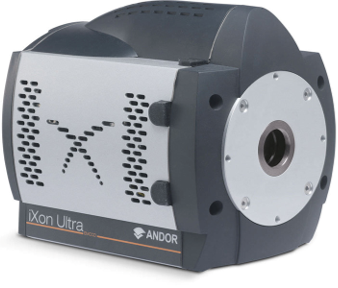
\includegraphics[scale=0.27]{Figures/iXon-Ultra-897.png}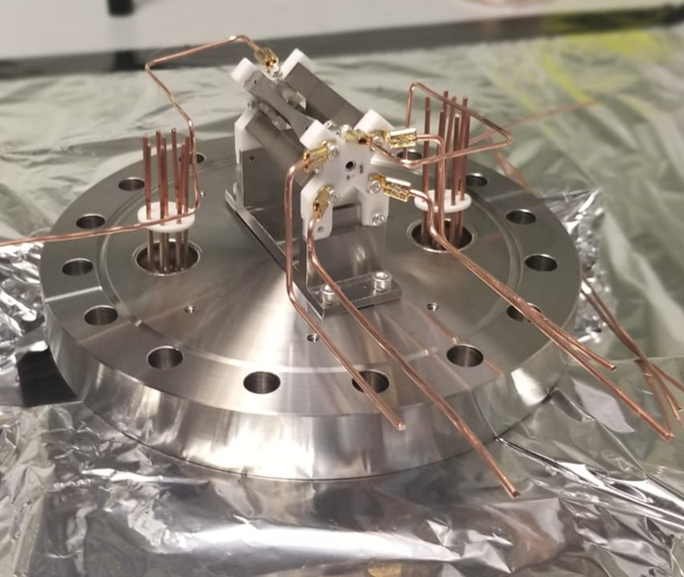
\includegraphics[scale=0.18]{Figures/ion_trap_photo.png}} % Optional title page image, comment this line to remove it

\institute{Imperial College London}

\date{16/07/2019}

%------------------------------------------------

\begin{document}

%------------------------------------------------

\begin{frame}
	\maketitle % Automatically created using the information in the commands above
\begin{picture}(0,0) 
    % \put{} defines the position of the frame
    \put(240,240){\makebox(20,40)[bl]{
    
\includegraphics[scale=0.5]{Figures/IC_logo.png}
    }}%
  \end{picture}%
\end{frame}

%----------------------------------------------------------------------------------------
%	 SECTION 1
%----------------------------------------------------------------------------------------

%\section{Section 1} % Section title slide, unnumbered

%------------------------------------------------



%------------------------------------------------
\begin{frame}{Overview}

\begin{itemize}
\item Iontraps and EMCCD Cameras
\bigskip
\item Motivation and Aims of the Project
\bigskip
\item Current Progress
\bigskip
\item Future plans
\end{itemize}

\end{frame}

%------------------------------------------------
\begin{frame}[noframenumbering]


Iontraps and EMCCD Cameras



\end{frame}



%------------------------------------------------
\begin{frame}{Ion traps}

\begin{itemize}
\item An ion trap is a device that is used to levitate small clouds of ions, or  a single atomic ion, in free
space, inside a vacuum chamber.
\bigskip
\item For example a Penning trap confines the motion of the ions through the use of static electric and magnetic fields
\end{itemize}

\end{frame}

%------------------------------------------------
\begin{frame}{EMCCD Cameras}

\begin{itemize}
\item A Charged Coupled Devide (CCD) is a silicon based semiconductor chip  which captures light and converts the photons to digital data in the form of electrons
\bigskip
\item An Electron Multiplying CCD (EMCCD) has an identical structure to conventional CCDs but is more sensitive and capable of single photo detection
\bigskip
\item The shift register in EMCCDs are extended to include the Gain register which significantly improves low light detection
\end{itemize}

\end{frame}

%------------------------------------------------

\begin{frame}{EMCCD Cameras}

\begin{figure}
\centering
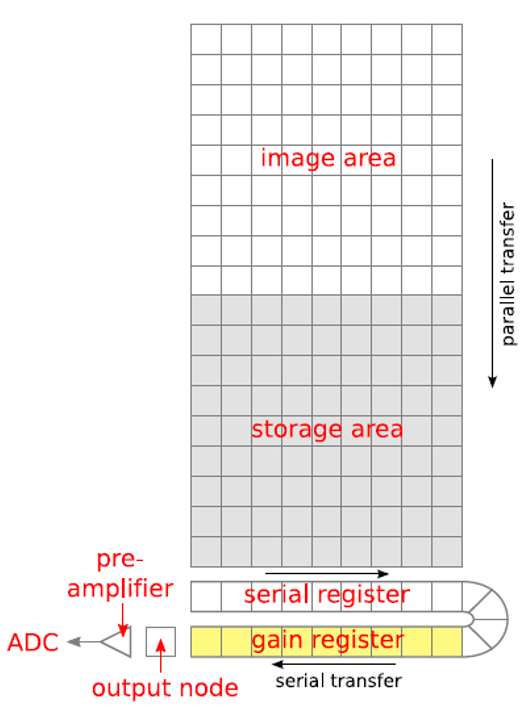
\includegraphics[scale=0.4]{Figures/EMCCD_Structure.PNG}
\end{figure}

\end{frame}

%------------------------------------------------
\begin{frame}[noframenumbering]

Motivation and Aims of the Project



\end{frame}



%------------------------------------------------
\begin{frame}{Motivation and Aims}

\begin{itemize}
\item Write a program in Python to interface an Andor iXon Ultra EMCCD camera used in ion trap
experiments.
\bigskip
\item Find a method of distinguishing between a bright ion and a dark ion
\bigskip
\item Find the setting of the program which takes the best images of the ions
\end{itemize}


\end{frame}

%------------------------------------------------
\begin{frame}[noframenumbering]

Current Progress



\end{frame}



%------------------------------------------------

\begin{frame}{The Program}

\begin{itemize}
\item Two separate programs were written in Python: one to control the EMCCD camera and take pictures of ion(s) and the other to load the images 
\bigskip
\item A Dynamic Link Library (DLL) containing various functions of the camera used by the program to control the camera
\bigskip
\item Both programs are object oriented and have its own graphical user interface (GUI) created using QT Creator software

\end{itemize}


\end{frame}

%------------------------------------------------
\begin{frame}{Camera Control Program}

\begin{figure}
\centering
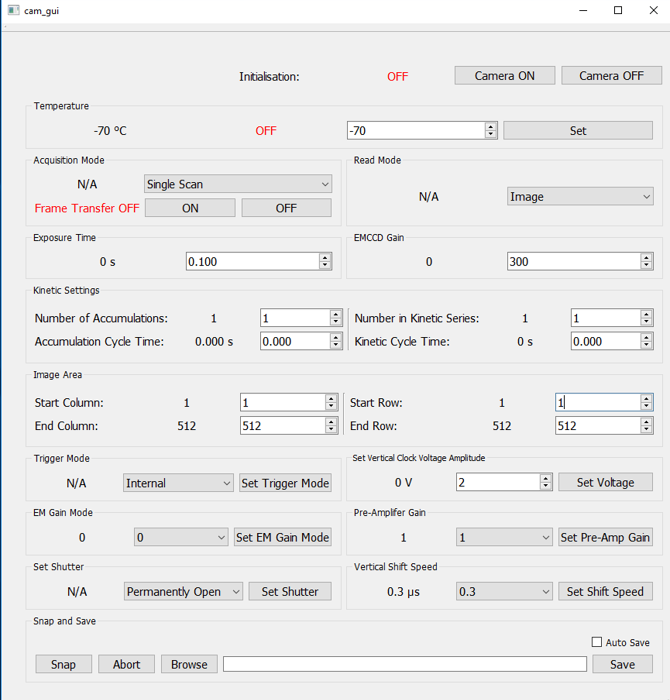
\includegraphics[scale=0.4]{Figures/cam_program.PNG}
\end{figure}


\end{frame}

%------------------------------------------------
\begin{frame}{Image Loading Program}

\begin{figure}
\centering
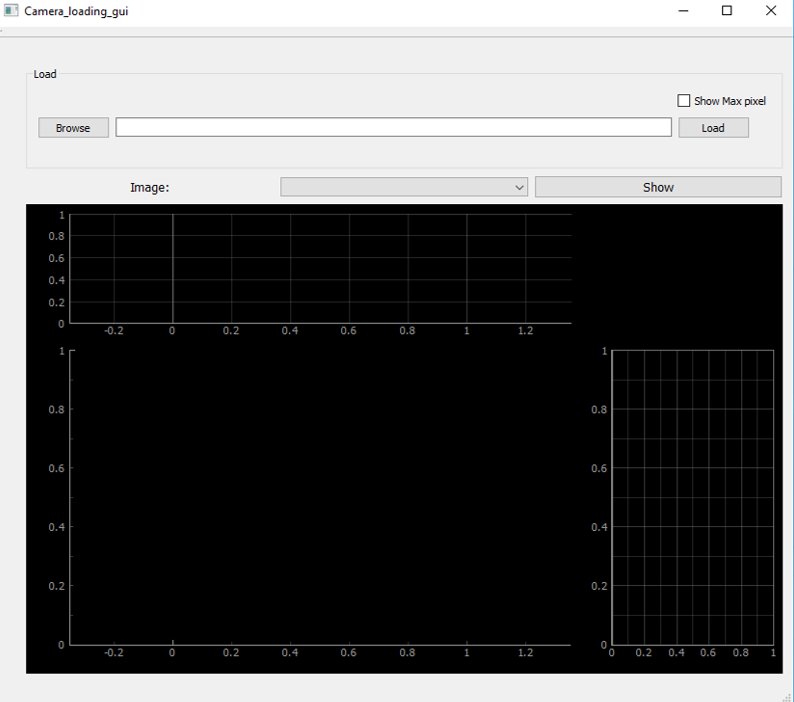
\includegraphics[scale=0.4]{Figures/pic_load_program.PNG}
\end{figure}


\end{frame}

%------------------------------------------------
\begin{frame}{Investigating Camera Properties}

\begin{itemize}
\item The camera control program was first tested with noise readings and compared with commercial software to ensure the python program is working as expected
\bigskip
\item The affect of the Exposure time and EMCCD gain on the mean noise reading per pixel were tested

\end{itemize}



\end{frame}

%------------------------------------------------
\begin{frame}{ Mean Signal Count vs. Exposure time}


\begin{figure}
\centering     
\subfigure[Python Program]{\label{fig:a}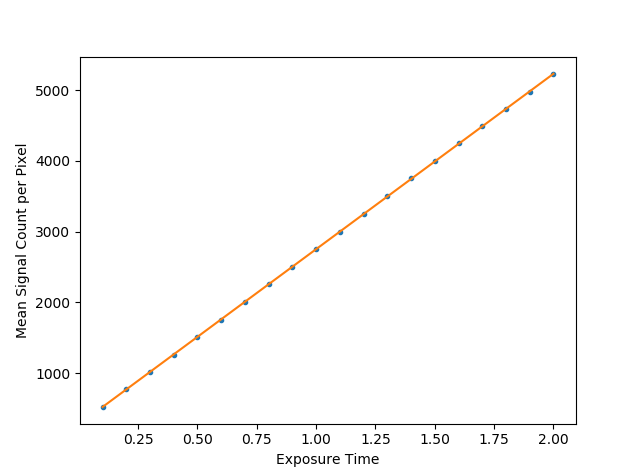
\includegraphics[width=55mm]{Figures/Noise_Python.png}}
\subfigure[Commercial Software]{\label{fig:b}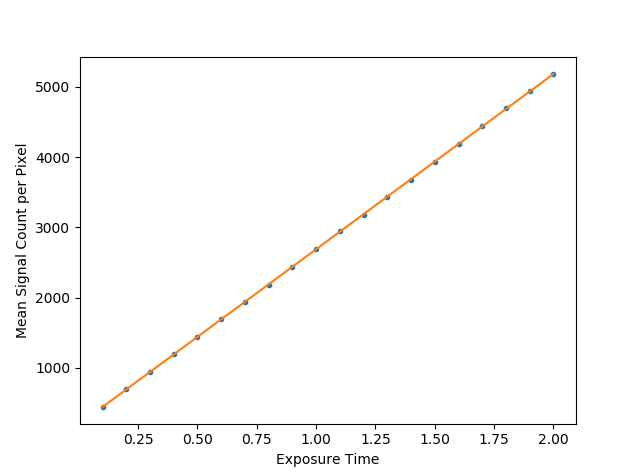
\includegraphics[width=55mm]{Figures/Noise_Commercial.png}}

\end{figure}


\end{frame}

%------------------------------------------------
\begin{frame}{ Mean Signal Count vs. EMCCD Gain}


\begin{figure}
\centering
\renewcommand{\thesubfigure}{(a)}     
\subfigure[Python Program]{\label{fig:a}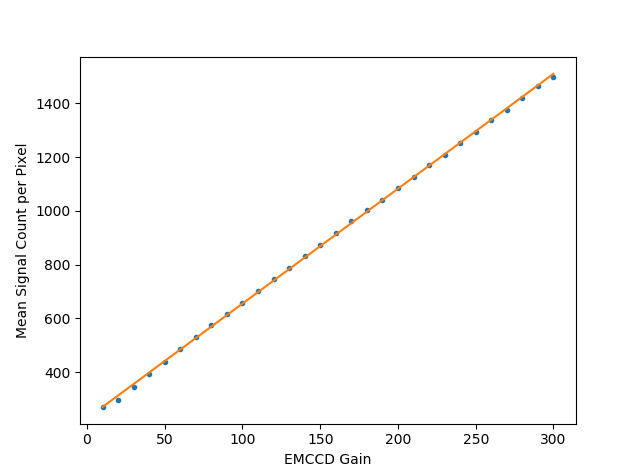
\includegraphics[width=55mm]{Figures/Gain_Python.png}}
\renewcommand{\thesubfigure}{(b)}     
\subfigure[Commercial Software]{\label{fig:b}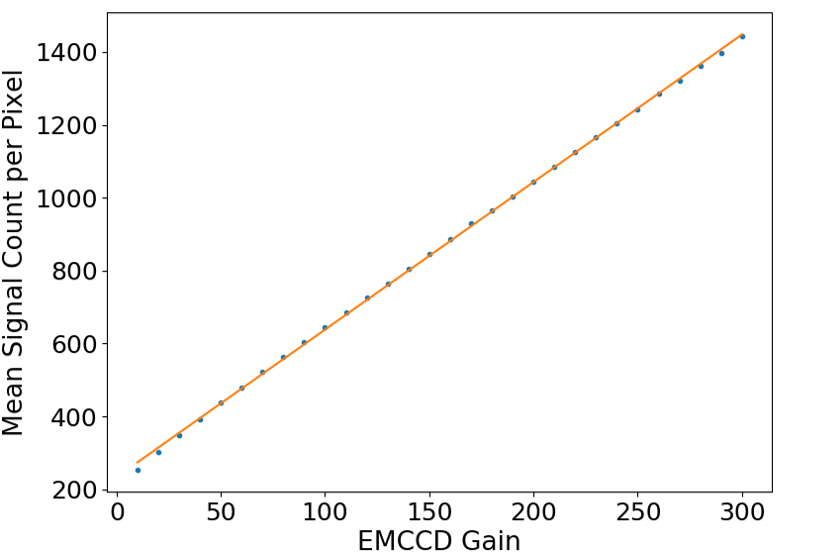
\includegraphics[width=55mm]{Figures/Gain_Commercial.png}}

\end{figure}


\end{frame}

%------------------------------------------------
\begin{frame}{Images of Single Ion at Different Exposure Times}



\begin{figure}
\centering
\renewcommand{\thesubfigure}{(a)}     
\subfigure[5 Second Exposure]{\label{fig:a}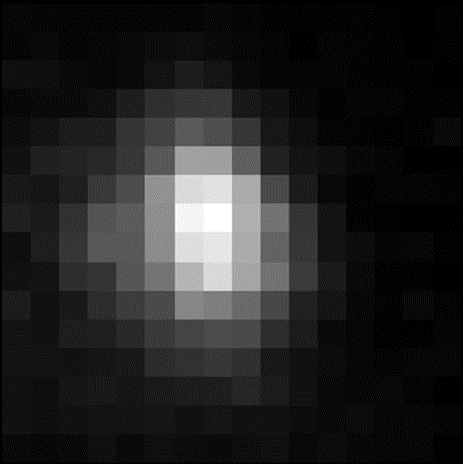
\includegraphics[width=36mm]{Figures/5_sec_exposure.png}}
\renewcommand{\thesubfigure}{(b)}     
\subfigure[2 Second Exposure]{\label{fig:b}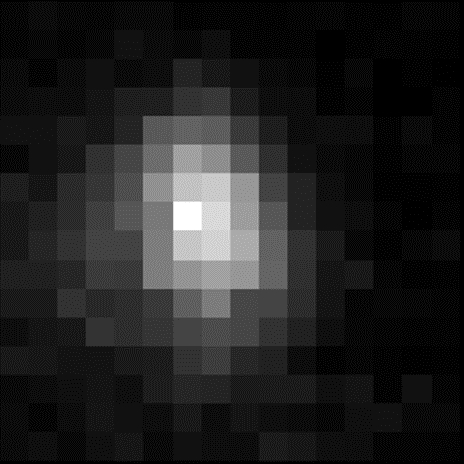
\includegraphics[width=36mm]{Figures/2_sec_exposure.png}}
\renewcommand{\thesubfigure}{(c)}     
\subfigure[1 Second Exposure]{\label{fig:c}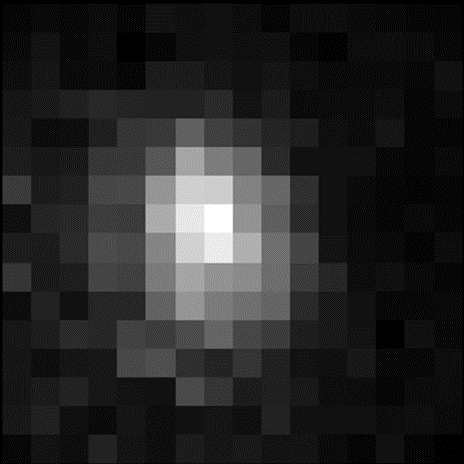
\includegraphics[width=36mm]{Figures/1_sec_exposure.png}}
\end{figure}


\end{frame}



%------------------------------------------------
\begin{frame}{Images of Single Ion at Different Exposure Times (cont.)}



\begin{figure}
\centering
\renewcommand{\thesubfigure}{(d)}     
\subfigure[0.7 Second Exposure]{\label{fig:d}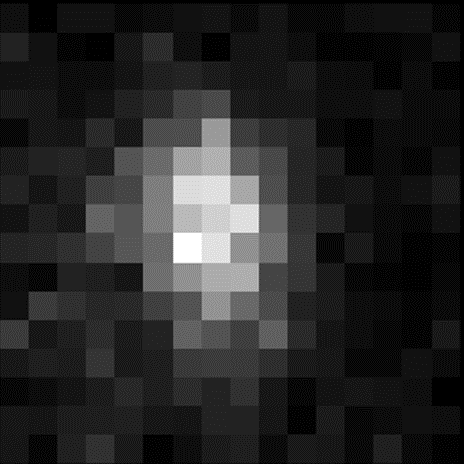
\includegraphics[width=36mm]{Figures/700ms_exposure.png}}
\renewcommand{\thesubfigure}{(e)}     
\subfigure[0.4 Second Exposure]{\label{fig:e}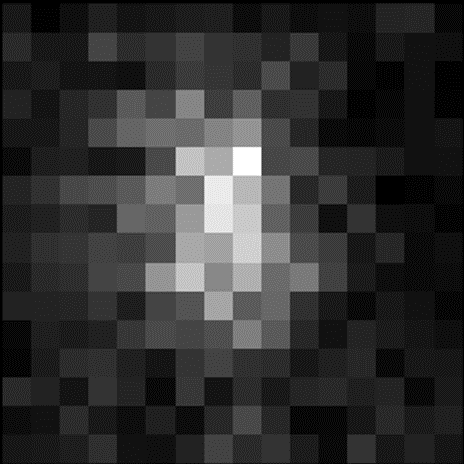
\includegraphics[width=36mm]{Figures/400ms_exposure.png}}
\renewcommand{\thesubfigure}{f)}     
\subfigure[0.1 Second Exposure]{\label{fig:f}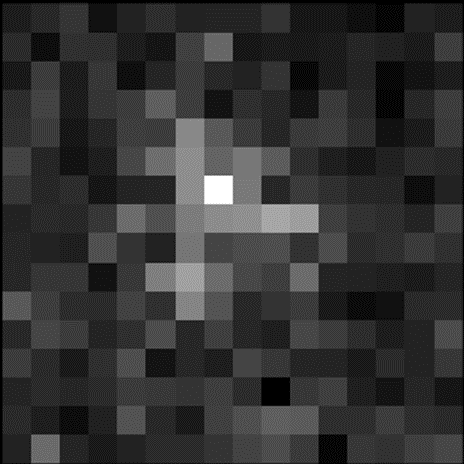
\includegraphics[width=36mm]{Figures/100ms_exposure.png}}
\end{figure}


\end{frame}



%------------------------------------------------
\begin{frame}[noframenumbering]

Future Plans



\end{frame}


%------------------------------------------------
\begin{frame}{Future Plans}

\begin{itemize}
\item Investigate the minimum exposure required for a bright ion to be able to be distinguished from a dark ion
\bigskip
\item A bright ion can no longer be distinguished from a dark ion if the distibution of the dark ion and bright ion signal counts have a large overlap

\end{itemize}

\begin{figure}
\centering
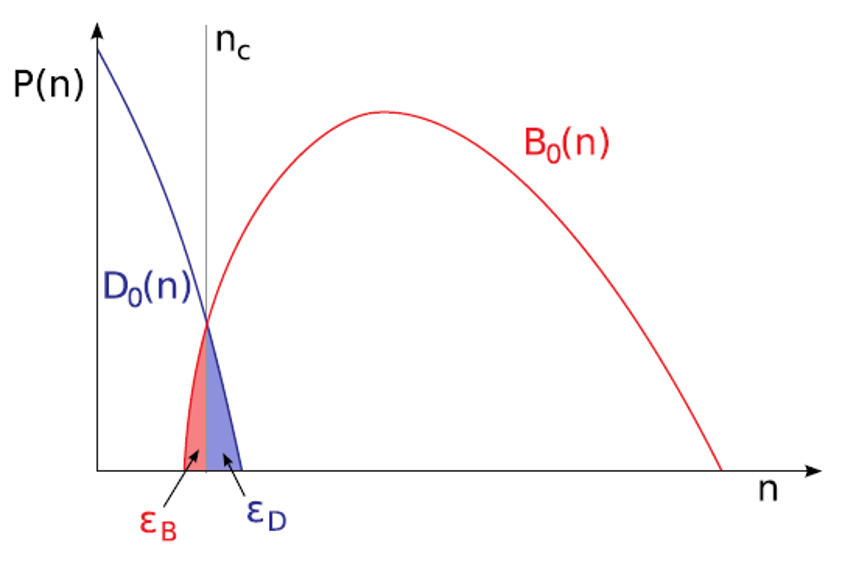
\includegraphics[scale=0.3]{Figures/B_D_graph.png}
\end{figure}

\end{frame}

%------------------------------------------------
\begin{frame}{Future Plans (cont.)}

\begin{itemize}
\item Comparing the differences in quality for image taken when the camera is externally triggered by the experiment and when the came camera triggers the experiment and the start of exposure
\bigskip
\item The EMCCD has a 'keep clean' cycle which clears the sensor to ensure it is charge free before the next exposure.
\bigskip
\item Externally triggering the camera may interupt the keep clean cycle and produce a more noisy image
\bigskip
\item The camera gives of a 'fire signal' during exposure which can be used to trigger the start of the experiment at the end of a 'keep clean' cycle
\end{itemize}


\end{frame}

%------------------------------------------------
\begin{frame}{Conclusions}

\begin{itemize}
\item A python program with a GUI was created to acquire pictures of fluorescence of single ions and another program was created to view the images and show the vertical and horizontal projections
\bigskip
\item A reliable method/algorithm is required to distinguish bright ions from dark ions at short exposure time
\bigskip
\item Find the camera triggering mode which gives images of highest signal to noise ratio

\end{itemize}


\end{frame}

%------------------------------------------------
\begin{frame}[noframenumbering]

\centering
Thank You for Listening!



\end{frame}


%------------------------------------------------


\end{document}
